\documentclass[11pt]{article}
\usepackage[sc]{mathpazo} %Like Palatino with extensive math support
\usepackage{fullpage}
\usepackage[authoryear,sectionbib,sort]{natbib}
\linespread{1.7}
\usepackage[utf8]{inputenc}
\usepackage{lineno}

%%%%%%%%%%%%%%%%%%%%%
% LaTeX packages
%%%%%%%%%%%%%%%%%%%%%
% Please be sparing in your use of additional LaTeX packages, and
% upload any required style files to Editorial Manager with the file
% type "LaTeX ancillary files (.sty, .bst)."
\usepackage{amsmath}
\usepackage{graphicx,epstopdf} %remove when remove figures

%%%%%%%%%%%%%%%%%%%%%
% Line numbering
%%%%%%%%%%%%%%%%%%%%%
\usepackage{lineno}
% Please use line numbering with your initial submission and
% subsequent revisions. After acceptance, please comment out 
% the commands \usepackage{lineno}, \linenumbers{} 
% and \modulolinenumbers[3] below.

\title{The temperature-size rule is predicted to stabilize the response of consumer-resource dynamics under warming\\
or\\
Temperature-dependent body size alters the effects of temperature on consumer resource dynamics}

%%%%%%%%%%%%%%%%%%%%%
% Authorship
%%%%%%%%%%%%%%%%%%%%%
% Please remove authorship information while your paper is under review,
% unless you wish to waive your anonymity under double-blind review. 
% Remember to uncomment the information after acceptance.

%\author{Matthew Miles Osmond$^{1,\ast}$ \\ 
%et al$^{2}$}

\date{}

\begin{document}

\maketitle

%\noindent{}1. Biodiversity Research Centre and Department of Zoology, University of British Columbia, Canada;
%
%\noindent{}2. others;
%
%\noindent{}$\ast$ Corresponding author; e-mail: mmosmond@zoology.ubc.ca.

\bigskip

\textit{Manuscript elements}: Figure~1, figure~2?, figure~3?, supplementary \texttt{Mathematica} file.
\bigskip

\textit{Keywords}: Metabolic theory, predator-prey, plant-herbivore, body size, allometry, functional response, mathematical model.

\bigskip

\textit{Manuscript type}: Note. 
% Or e-article, note, e-note, natural history miscellany,
% e-natural history miscellany, comment, reply, symposium, or
% countdown to 150.

\bigskip

\noindent{\footnotesize Prepared using the suggested \LaTeX{} 
template for \textit{Am.\ Nat.}}

\linenumbers{}
\modulolinenumbers[3]

\newpage{}

%%%%%%%%%%%%%%%%%%%%%%%%%%%%%%%%%%%%%%%%%%%%%%%%
\section*{Abstract}
%%%%%%%%%%%%%%%%%%%%%%%%%%%%%%%%%%%%%%%%%%%%%%%%
Body size influences the dynamical relationship between consumers and their resources. 
Mounting evidence suggests that body size declines with increasing temperature, a pattern called the temperature-size rule (TSR). 
The growing theory on temperature-dependent consumer resource interactions has yet to integrate the TSR into a general framework for how temperature affects consumer resource dynamics. 
We expanded an existing temperature-dependent consumer-resource model to include the indirect effects of warming, through changes in body size, and parameterized the model with data from data syntheses. 
We analyzed this model to answer the following questions: 
1) How does including the TSR affect predictions for how temperature affects consumer-resource stability and biomass ratios? 
2) Under what circumstances are the effects of the TSR most substantial? 
%3) Is the TSR predicted to induce a change in the functional response? 
We found that including the TSR led to two qualitatively different predictions: under warming i) consumer-resource biomass is no longer expected to decline and ii) the dynamics are expected to become more stable, as opposed to the decline in stability predicted without the TSR. 
These qualitatively different predictions were strengthened by asymmetric temperature-size responses and type-II functional responses.
Our analyses suggest that the effect of temperature on body size likely plays an important role in the response of consumer-resource systems to changing temperatures. 

\newpage{}

%%%%%%%%%%%%%%%%%%%%%%%%%%%%%%%%%%%%%%%%%%%%%%%%
\section*{Introduction}
%%%%%%%%%%%%%%%%%%%%%%%%%%%%%%%%%%%%%%%%%%%%%%%%

% The journal does not have numbered sections in the main portion of
% articles. Please refrain from using section references such as
% section~\ref{section:CountingOwlEggs}, and refer to sections by name
% (e.g. section ``Counting Owl Eggs'').

% Please note that we prefer (\citealt{Xiao2015}) to \citealt{Xiao2015},
% since \citealt{} inserts a comma after "et al."

%%%%%%%%%%%%%%%%%%%%%%%%%%%%%
%my little weekend attempt

%Temperature and body size determine many biological rates (\cite{West1997,Gillooly2001}).
%How these factors individually influence consumer-resource dynamics has already been demonstrated (\cite{Gilbert2014,DeLong2015}).
%How they act in symphony has not yet been investigated.
%
%Temperature also affects body size through the temperature-size rule (\cite{Atkinson1994}).
%Thus, temperature directly and indirectly affects ecosystem dynamics.
%These two pathways have the potential to reinforce or counteract one another, with population level consequences.
%
%Here we model a simple consumer-resource interaction, with population dynamic parameters that depend on temperature and body size, and body sizes that depend on temperature.
%We ask how including dependencies on both temperature and body size, as well as incorporating the temperature-size rule, affects the response of the consumer-resource dynamics to increasing temperature.

%%%%%%%%%%%%%%%%%%%%%%%%%%%%%

Populations of consumers and their resources are joined across time by the fact that energy to the consumer comes from the resource, and the consumer determines mortality rates of the resource. 
In these systems, temperature-dependent consumption, growth and mortality rates can change the dynamics and their outcomes. 
Through the temperature-dependence of metabolism (\cite{West1997,Gillooly2001}) and hence demographic vital rates, small changes in temperature that are not necessarily physiologically stressful for organisms can translate to changes in the stability and coexistence of consumers and their resources, producing predictable but non-intuitive effects of warming on simple food webs (\cite{Gilbert2014,Vasseur2005,OConnor2011,Rall2010}). 

Demographic rates and consumer-resource interactions also depend on body size (\cite{Yodzis1992,DeLong2015}). 
Not only do rates of growth, mortality and consumption scale predictably with individual body sizes, but the consumption rates of consumer-resource systems can also depend on the ratio of body masses between consumers and prey (\cite{Kalinkat2013}). 
Changes in body size or body size ratios can therefore change demographic and interaction rates. Given the importance of body size to the dynamics and outcomes of consumer-resource interactions, frameworks for understanding how temperature affects consumer-resource dynamics have not considered the importance of changes in body size with temperature.

The frequently-observed negative relationship between temperature and body size, the temperature-size rule (TSR), has been called the third universal response to warming (\cite{Gardner2011}). 
For comparisons within populations, among species and across biogeographic gradients, body size of ectotherms tends to decline with increasing temperature (\cite{Atkinson1994,Daufresne2009,Forster2012,DeLong2012}). 
Although the mechanism for declining body size with warming varies among examples, including physiological plasticity, selection for smaller individuals, and turnover in species composition, the pattern is similar across levels of organization (\cite{Forster2012}). 
\cite{Forster2012} reported a mean slope of -3.65$\%/ ^\circ C$ for aquatic organisms, ranging from -1.80$\% / ^\circ C$ for unicells, and becoming stronger (more negative) in increasingly large aquatic multicelled organisms.

Because body size is so central to consumer-resource dynamics, such a systematic pattern of changing body size with temperature could alter predictions for how temperature affects stability, persistence and coexistence in consumer-resource systems. 
We therefore integrated the temperature size rule into a general framework for temperature-dependent consumer-resource interactions to answer the following questions: 
1) How does the TSR affect stability and consumer:resource biomass ratios over a temperature gradient?, 
2) Does the effect of the TSR depend on whether consumer and resource body sizes respond similarly to temperature?, 
3) Does the effect of the TSR depend on the form of the functional response?, 
And finally, 4) does the TSR itself induce a change in the functional response?

%%%%%%%%%%%%%%%%%%%%%%%%%%%%%%%%%%%%%%%%%%%%%%%%%%%
\section*{Methods and results}
%%%%%%%%%%%%%%%%%%%%%%%%%%%%%%%%%%%%%%%%%%%%%%%%%%%

%%%%%%%%%%%%%%%%%%%%%%%%%%%
\subsection*{The underlying consumer-resource dynamics}

We begin, like \cite{Gilbert2014}, with the Rosenzweig-MacArthur equations (\cite{Rosenzweig1963})
\begin{equation}\label{eq:RM}
\begin{aligned}
\frac{\mathrm{d}R}{\mathrm{d}t} =& r R \left(1 - \frac{R}{K} \right) - f(R) R C\\
\frac{\mathrm{d}C}{\mathrm{d}t} =& e f(R) R C - m C,
\end{aligned}
\end{equation}
which describe the rates of change in total resource $R\in[0,K]$ and consumer $C\geq0$ biomass with time $t$.

In the absence of consumers, $C=0$, the resource grows logistically, with intrinsic growth rate $r\geq0$ and carrying capacity $K>0$.
The intrinsic growth rate describes the rate at which resource biomass increases without consumers when the resource is rare, $R\approx0$.
The carrying capacity is the equilibrium biomass of the resource without consumers.

Resource biomass is consumed by consumers at a rate $f(R) R C$, where $f(R)\geq0$ is called the functional response.
Of the biomass consumed, the unitless conversion efficiency parameter $e\in[0,1]$ determines the proportion of resource biomass that is directly converted into consumer biomass.
Consumers die at constant per capita mortality rate $m\geq0$.

An equilibrium is reached when the two rates of change in Equation \eqref{eq:RM} are zero, and solving the system at this point gives equilibrium resource $\hat{R}$ and consumer $\hat{C}$ biomass.
There are three equilibria for this system: total extinction $(R,C) = (0,0)$, consumer extinction $(R,C)=(K,0)$, and coexistence $(R,C)=(\hat{R},\hat{C})$, the latter with $\hat{R}>0$ and $\hat{C}>0$.
We are primarily concerned with the latter equilibrium, as that is presumably the equilibrium current consumer-resource systems are near.
At this coexistence equilibrium one can calculate the ratio of consumer to resource biomass, $\hat{C}:\hat{R}$, and also perform a linear stability analysis to derive the leading (largest in absolute value) eigenvalue $\lambda$, which determines if (and how readily) the system, when perturbed a small amount from this equilibrium, will return to it (see the supplementary \texttt{Mathematica} file for details).
Our measure of stability will be the negative of the real part of the leading eigenvalue.
The system is stable if and only if this value is positive, and the system will return to equilibrium faster when this value is larger (i.e., larger positive values imply ``more stable" systems).
Together these two measures tell us how biomass is partitioned and how stable this partitioning is.

As explained in \cite{Gilbert2014}, two aggregates well describe the dynamics of this system.
The first is $m /(e f(R))$, which describes (the inverse of) consumer growth, is the slope of the consumer zero-net growth isocline, and is the equilibrium abundance of resources at the coexistence equilibrium.
The second aggregate is $K$, the equilibrium resource biomass in the absence of consumers.
Dividing the second aggregate by the first gives a measure that defines the biomass potential of the resource that is converted into consumer biomass, $B_{CR} = e f(R) K / m$.
%Note that we have modified the presentation of \cite{Gilbert2014} by subsuming $R$ into $f(R)$ such that $f(R)$ is  a rate and thus more easily interpreted.
%This does not alter the results.

In what follows we will examine how our three measures, $B_{CR}$, $\hat{C}:\hat{R}$, and stability, change with temperature.
We start by assuming a type-I functional response, $f(R) = a$, where $a$ is called the attack rate, which describes the rate of resource consumption per resource biomass.
We later explore the effect of a type-II functional response and the potential for the functional response to change with temperature.

%%%%%%%%%%%%%%%%%%%%%%%%%%%
\subsection*{Adding temperature dependence}

\cite{Gilbert2014} discuss what is known about the temperature dependencies of $r$, $K$, $a$, $m$, and $e$, and give equations and parameter estimates in their Table 1.
Briefly, resource growth rate $r$ is expected to scale with metabolism as a Boltzmann-Arrhenius factor, $r(T) = r_0 \exp(-E_B/(kT))$, where $E_B$ is the activation energy of the metabolism $B$ (in units of eV), $k$ is Boltzmann's constant ($\approx 8.62 \times 10^{-5}$ eV/K), and $T$ is the temperature (in Kelvins).
Resource carrying capacity $K$ is determined by the ratio of the supply rate of nutrients into the system and the rate of uptake of nutrients by the resource, $r$.
With supply rate also scaling as a Boltzmann-Arrhenius factor with activation energy $E_S$, carrying capacity is  $K(T) = K_0 \exp(-(E_S - E_B)/(kT))$. 
Attack rate $a$ depends on the temperature dependence of the body velocities $\nu$ in both species, which both scale as Boltzmann-Arrhenius factors with activation energies $E_{\nu,i}$, with $i=\{R,C\}$.
Attack rate is then $a(T) = a_0 \sqrt{\sum \left[\nu_{0,i} \exp(-E_{\nu,i}/(kT)) \right]^2}$, where the sum is over $i=\{R,C\}$ and $\nu_{0,i}$ are rate-constants.
Consumer mortality is also expected to scale as a Boltzmann-Arrhenius factor, $m(T) = m_0 \exp(-E_m/(kT))$.
Conversion efficiency is assumed to be independent of temperature $e(T) = e_0$.

The black curves in Figure \ref{AllTempMassDep} show $B_{CR}$, equilibrium consumer to resource biomass ratio $\hat{C}:\hat{R}$, and stability of the coexistence equilibrium as functions of temperature $T$ (plotted in Celsius).
In these plots $r$, $K$, $a$, and $m$ all depend on temperature as discussed above, unlike Figure 3 in \cite{Gilbert2014} where only $K$ depends on temperature and the rest of the parameters are held constant.
Comparing with Figure 3 in \cite{Gilbert2014} shows that adding temperature dependence in $r$, $a$, and $m$ causes equilibrium consumer:resource biomass to decline with temperature (instead of increasing) and stability to decrease at a slower rate  with increasing temperature.
These changes are largely driven by the temperature dependence of consumer mortality: increasing temperature increases consumer mortality, lowering equilibrium consumer biomass and increasing stability at high temperatures (relative to the case where mortality $m$ does not depend on temperature).

%%%%%%%%%%%%%%%%%%%%%%%%%%%
\subsection*{Adding mass dependence and the temperature size-rule}

We next allow the population dynamic parameters to depend on the body size of the interacting species.
Following \cite{DeLong2015}, each parameter can be written as a power law function of the body mass of resource $M_R$ or consumer $M_C$.
Here we combine \cite{DeLong2015} and \cite{Gilbert2014} by letting the parameters depend on both temperature and mass: $r(T, M_R) = r(T) M_R^\rho$, $K(T, M_R) = k(T) M_R^\kappa$, $a(T, M_C) = a(T) M_C^\alpha$, $e(T, M_C) = e(T) M_C^\epsilon$, and $m(T, M_C) = m(T) M_C^\mu$.

If mass does not change with temperature then adding these mass dependencies does not change the response of the consumer-resource dynamics to temperature.
However, mass is expected to change with temperature, according to the temperature-size rule (\cite{Atkinson1994}).
%For organisms with a dry mass of less than $10^{-3}$ mg body mass declines linearly with temperature.
We incorporate a simple form of the temperature-size rule here for illustrative purposes.
In particular, we assume body mass declines linearly with temperature, $M_i(T) = M_i(T_{ref}) (1 - \beta_i (T - T_{ref})$, where $\beta_i$ is the fraction that mass is reduced as temperature is increased by one degree and $T_{ref}$ is a reference temperature, which we set to 15$^\circ C$ throughout.
This linear decline best approximates the response of organisms with a dry mass of less than $10^{-3}$ mg, whereas larger organisms experience a faster than linear decline (\cite{Forster2012}).

The red curves in Figure \ref{AllTempMassDep} depict our main results: adding mass dependencies and the temperature-size rule modifies our prediction of how consumer-resource dynamics respond to changes in temperature.
While there is little change in $B_{CR}$, the equilibrium consumer to resource biomass ratio is no longer expected to decline with increasing temperature and stability is now expected to increase.
These changes are brought on by the indirect effect of temperature, through mass, on the population dynamic parameters.
In particular, the lack of decline in the consumer to resource biomass ratio with the temperature-size rule, relative to the case without it, is primarily driven by changes in consumer conversion efficiency and the intrinsic growth rate of the resource.
Both of these rates increase with declining body mass, supporting a larger consumer biomass, relative to resource biomass. 
The indirect effects of temperature, through body size, act in opposition to the direct effects of temperature, and in the case of stability the indirect effects override the direct effects to produce a qualitatively different prediction.
%The increase in stability with the temperature-size rule stimulates the tantalizing possibility that its existence is adaptive, although obviously much more careful thought is needed here.

%%%%%%%%%%%%%%%%%%%%%%%%%%%
\subsection*{Exploring asymmetric temperature-size responses}

In Figure \ref{AllTempMassDep} we assumed both resource and consumer body mass declined with temperature at the same rate, $\beta_C = \beta_R = 0.02$, i.e., both decline $2\%$ per degree increase.
However, larger organisms often experience larger declines in body size with temperature (\cite{Forster2012}).
%In Figure \ref{AllTempMassDepAsymm} we let consumer body size decline twice as fast as the resource, $2 \beta_R = \beta_C = 0.04$.
In the supplementary \texttt{Mathematica} file we let consumer body size decline twice as fast as the resource, $2 \beta_R = \beta_C = 0.04$.
The main effect of the asymmetric temperature-size response is that i) the $B_{CR}$ with $E_S > E_B$ now asymptotes at higher temperatures (compare with the dark solid curves in Figure \ref{AllTempMassDep}) and ii) stability now increases even faster with increasing temperature.

%%%%%%%%%%%%%%%%%%%%%%%%%%%
\subsection*{Type-II functional response}

The consumption of resources in some systems may be better described by a type-II functional response, $f(R) = b / (1 + b h R)$, where $b$ is sometimes called the capture rate (per resource biomass per consumer biomass rate of resource biomass consumption) and $h$ is the handling time.
This collapses to a type-I functional response at low resource biomass, $f(R) \approx b$ for $R << 1/(b h)$.
And at high resource biomass a type-II functional response implies that the rate of resource consumption per consumer biomass asymptotes at $\lim_{R\rightarrow\infty}f(R) R = 1/h$, describing satiation of the consumer.

Both capture rate and handling time are known to depend on temperature and body mass.
In particular, capture rate scales like $b(T, M_R, M_C) = b_0 M_R^{b_R} M_C^{b_C} \exp(-E_b/(k T))$ and handling time like $h(T, M_R, M_C) = h_0 M_R^{h_R} M_C^{h_C} \exp(-E_h/(k T))$ (\cite{Rall2012}).
Using these dependencies and the parameter values in \cite{Rall2012} we can again plot $B_{CR}$, $\hat{C}:\hat{R}$, and stability as functions of temperature, this time with a type-II functional response.
We do this in the supplementary \texttt{Mathematica} file.
The main conclusions are: in comparison to a type-I functional response, a type-II functional response i) makes the $B_{CR}$ slopes more positive (increasing the response temperature when $E_S > E_B$), ii) makes equilibrium biomass ratios increase with temperature, and iii) makes stability increase more quickly with temperature.

As an aside, in this analysis we set $b_0$ to give $f(R) = 0.1$ at 15$^\circ C$, to remain consistent with \cite{Gilbert2014}.
This leaves $h_0$ as a free parameter. 
However, this free parameter only influences the results in the case of stability.
When $h_0$ is small enough to allow a stable coexistence equilibrium ($h_0 < 1\approx 0^{-12}$) we find that stability increases exponentially with temperature (see supplementary \texttt{Mathematica} for details).

\cite{Rall2012} complied a large database on capture rates and handling times and compared the data to their theoretical predictions.
They were surprised to find capture rate and handling time responded less strongly to temperature than expected (see their Figure 2a,d).
Interestingly, we found that the temperature-size rule reduces the sensitivity of both capture rate and handling time to temperature (see supplementary \texttt{Mathematica} file for details), and hence may explain the discrepancies observed between data and theory (\cite{Rall2012}). 

%%%%%%%%%%%%%%%%%%%%%%%%%%%
\subsection*{A functional response that depends on the body size ratio}

The functional response tends to be more type-II when consumers and resources have similar body sizes, but becomes more sigmoidal and hence more type-III when consumers are much bigger than their resource, as resources are then better able to hide when rare (\cite{Kalinkat2013}).
Without the temperature-size rule, the body mass ratio remains constant with temperature, and therefore the form of the functional response is not expect to change.
However, with the temperature-size rule body sizes change.
When the temperature-size responses are asymmetric, the ratio of body sizes will change and influence the form of the functional response.
Because consumers are often larger than their resource, and because larger organisms are expected to have greater reductions in body size with temperature, the ratio of consumer to resource body size will often decrease with temperature.
As stated above, lower consumer to resource body size ratios produce functional responses more like type-II, which are less stable than type-III functional responses, and hence the temperature-size rule can be said to destabilize the consumer-resource dynamics at high temperatures through this mechanism (and stabilize the dynamics at lower temperatures).
However, the amount by which the shape of the functional response is adjusted by the temperature-size rule does not appear to be large and therefore the stabilizing effects discussed in previous sections will likely prevail (see supplementary \texttt{Mathematica} file for details). 

%%%%%%%%%%%%%%%%%%%%%%%%%%%%%%%%%%%%%%%%%%%%%%%%%%%
\section*{Discussion}
%%%%%%%%%%%%%%%%%%%%%%%%%%%%%%%%%%%%%%%%%%%%%%%%%%%

%%%%%%%%%%%%%%%%%%%%%
% Acknowledgments
%%%%%%%%%%%%%%%%%%%%%
% You are encouraged to remove the Acknowledgments section while
% your paper is under review (unless you wish to waive your anonymity
% under double-blind review) if the Acknowledgments reveal your
% identity. If you remove this section, you will need to add it back
% in to your final files after acceptance.

%\section*{Acknowledgments}
%Stilianos!

%%%%%%%%%%%%%%%%%%%%%%%%%%%%%%%%%%%%%%%%%%%%%%%%%%%
\bibliographystyle{amnatnat}
\bibliography{library}


\newpage{}

%%%%%%%%%%%%%%%%%%%%%
% Figure legends
%%%%%%%%%%%%%%%%%%%%%
% Please include all figure legends in a separate section at the end of 
% the document. If you use \label{} and \ref{} to refer to your figures,
% these can still work even if you comment out the %includegraphics{}
% line. If you refer to figures as "fig. 1" (etc.) manually, the
% legends can also appear simply as paragraphs.
% For submission, please upload the relevant figure files separately to
% Editorial Manager; Editorial Manager should insert them at the end of
% the PDF automatically.
% Figure legends should be concise, though they can be longer than the
% titles of tables.

\section*{Figure legends}

%%%%%%%%%%%%%%%%%%%%%%%%%%%%%%%%%%%%%%%%%%%%%%%%
%\begin{figure}[!ht]
%\centering
%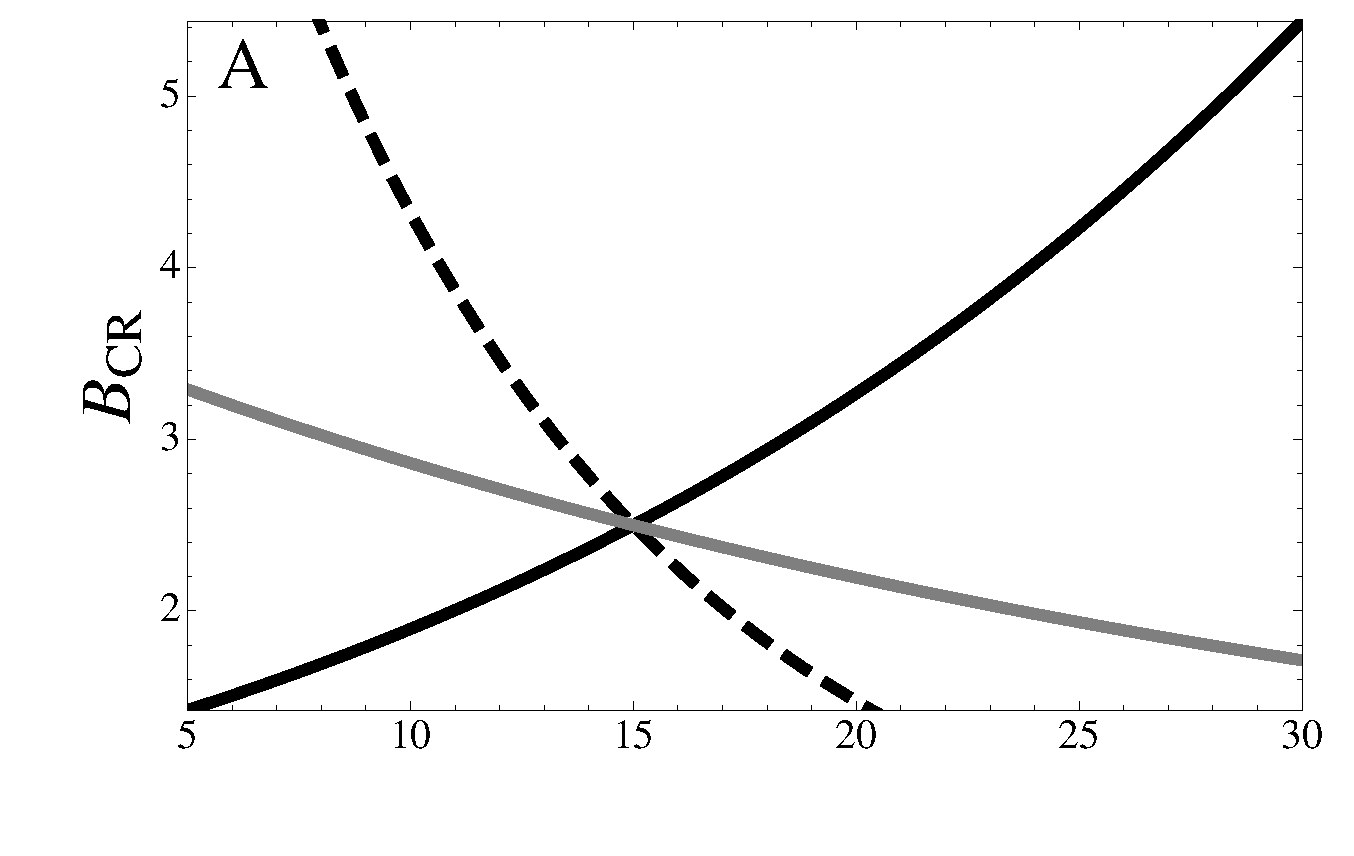
\includegraphics[width=0.5\linewidth]{BCRAllTempDep}
%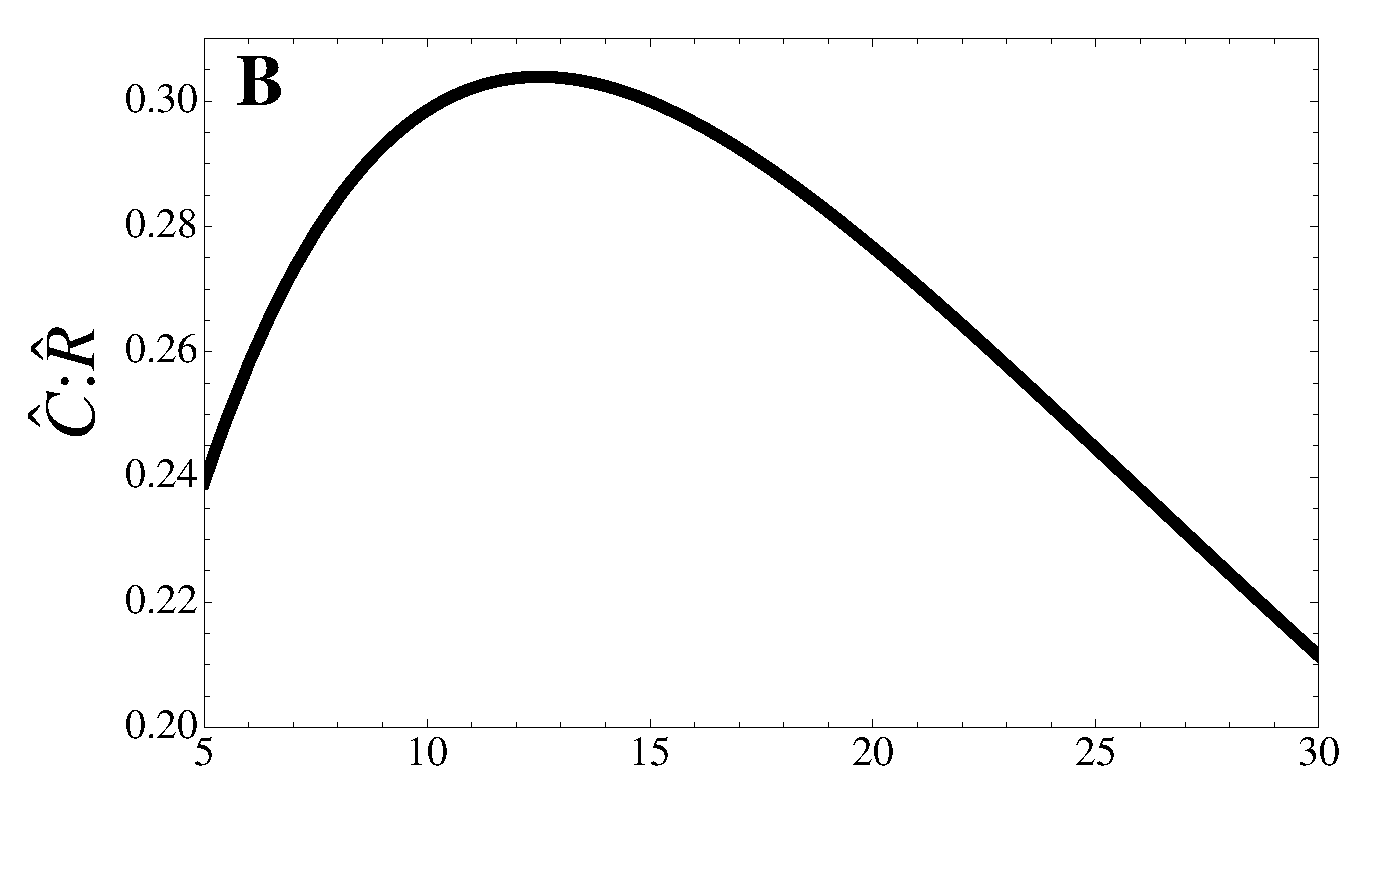
\includegraphics[width=0.5\linewidth]{CtoRAllTempDep}
%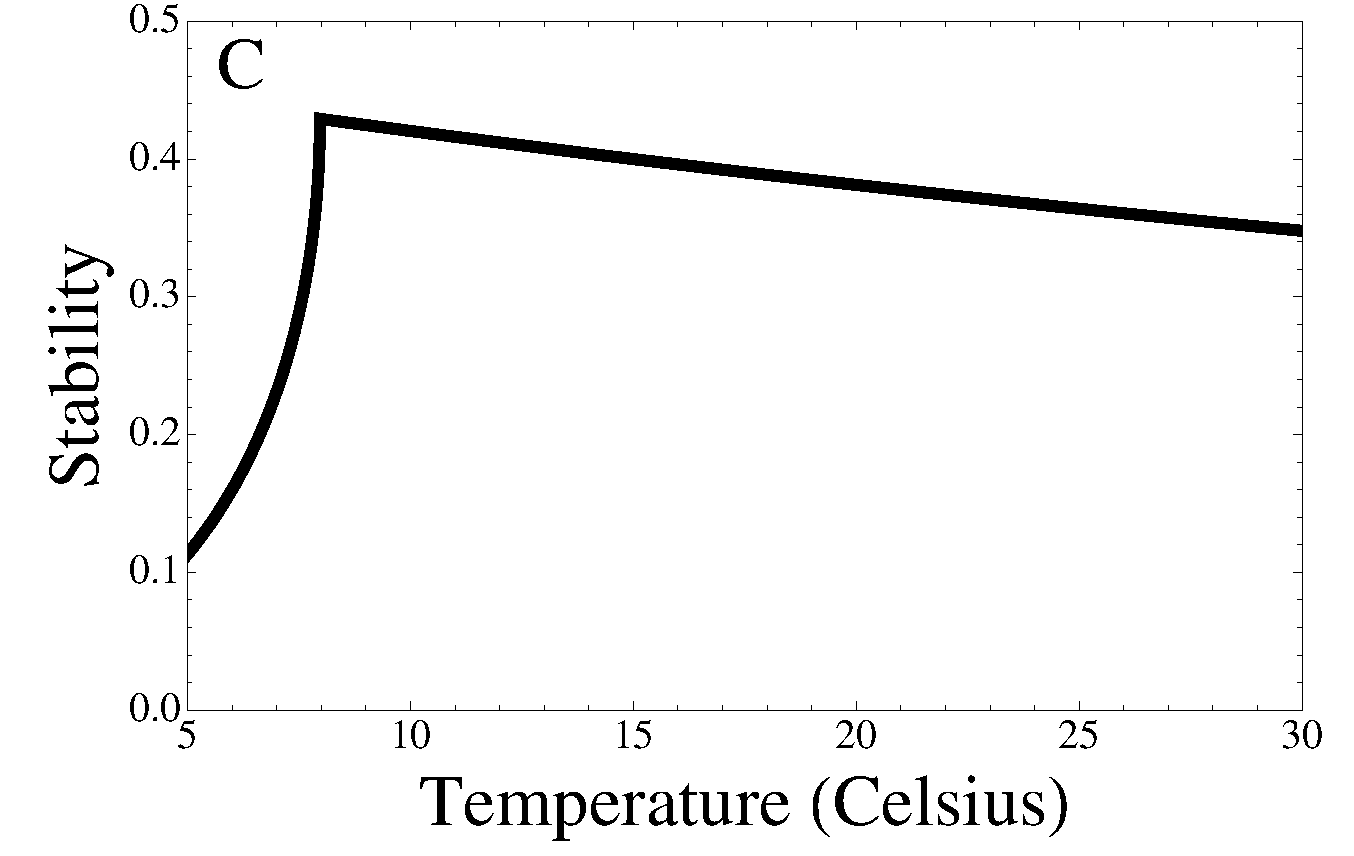
\includegraphics[width=0.5\linewidth]{StabilityAllTempDep}
%\caption{
%$B_{CR}$, equilibrium consumer to resource biomass ratio $\hat{C}:\hat{R}$, and stability of the coexistence equilibrium as functions of temperature $T$ (plotted in Celsius).
%Rate-constants (e.g., $r_0$) were chosen to make $r = 2$, $K = 100$, $a = 0.1$, $m = 0.6$, and $e = 0.15$ at 15$^\circ C$ (as in \cite{Gilbert2014}).
%Other parameters: $E_B = 0.32$ (solid black), $E_B = 0.9$ (dashed and gray), $E_S = 0.9$ (solid black and gray), $E_S = 0.32$ (dashed), $E_m = 0.65$, $E_{\nu,i} = 0.46$, $\nu_{0,i} = 1$.  
%}
%\label{AllTempDep}
%\end{figure}

%%%%%%%%%%%%%%%%%%%%%%%%%%%%%%%%%%%%%%%%%%%%%%%%
\begin{figure}[!ht]
\centering
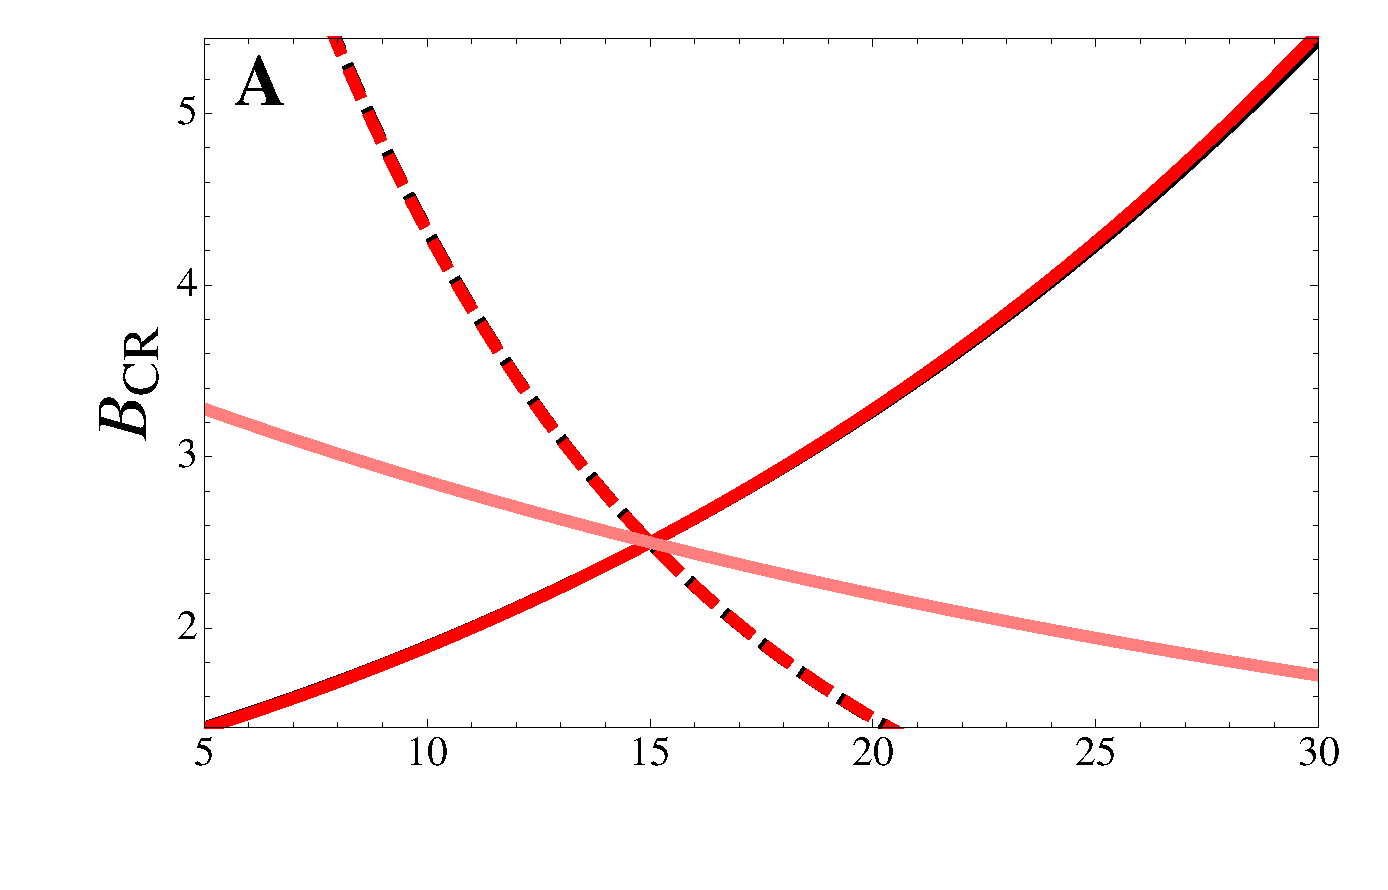
\includegraphics[width=0.5\linewidth]{BCRAllTempMassDep}
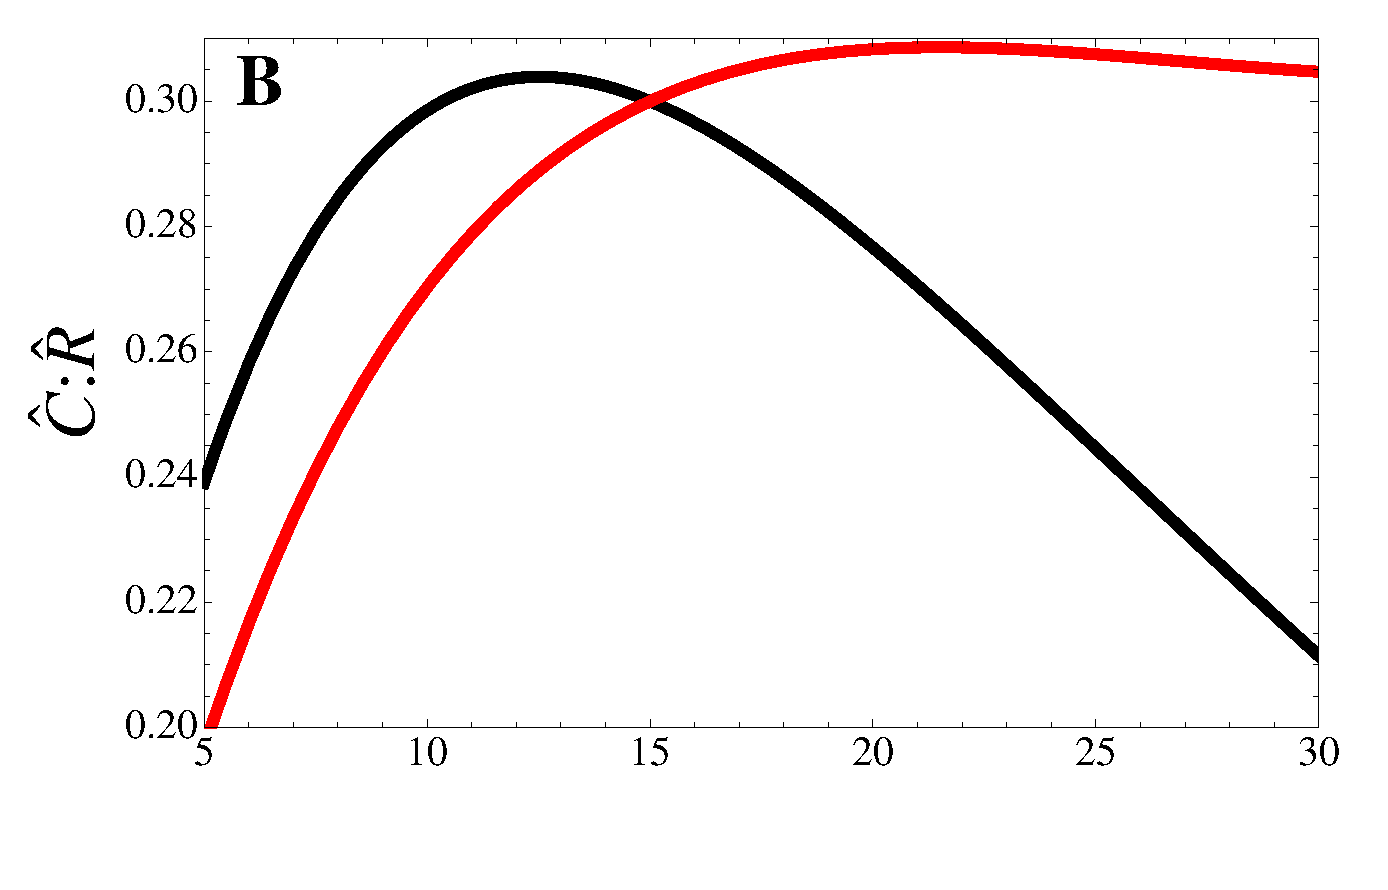
\includegraphics[width=0.5\linewidth]{CtoRAllTempMassDep}
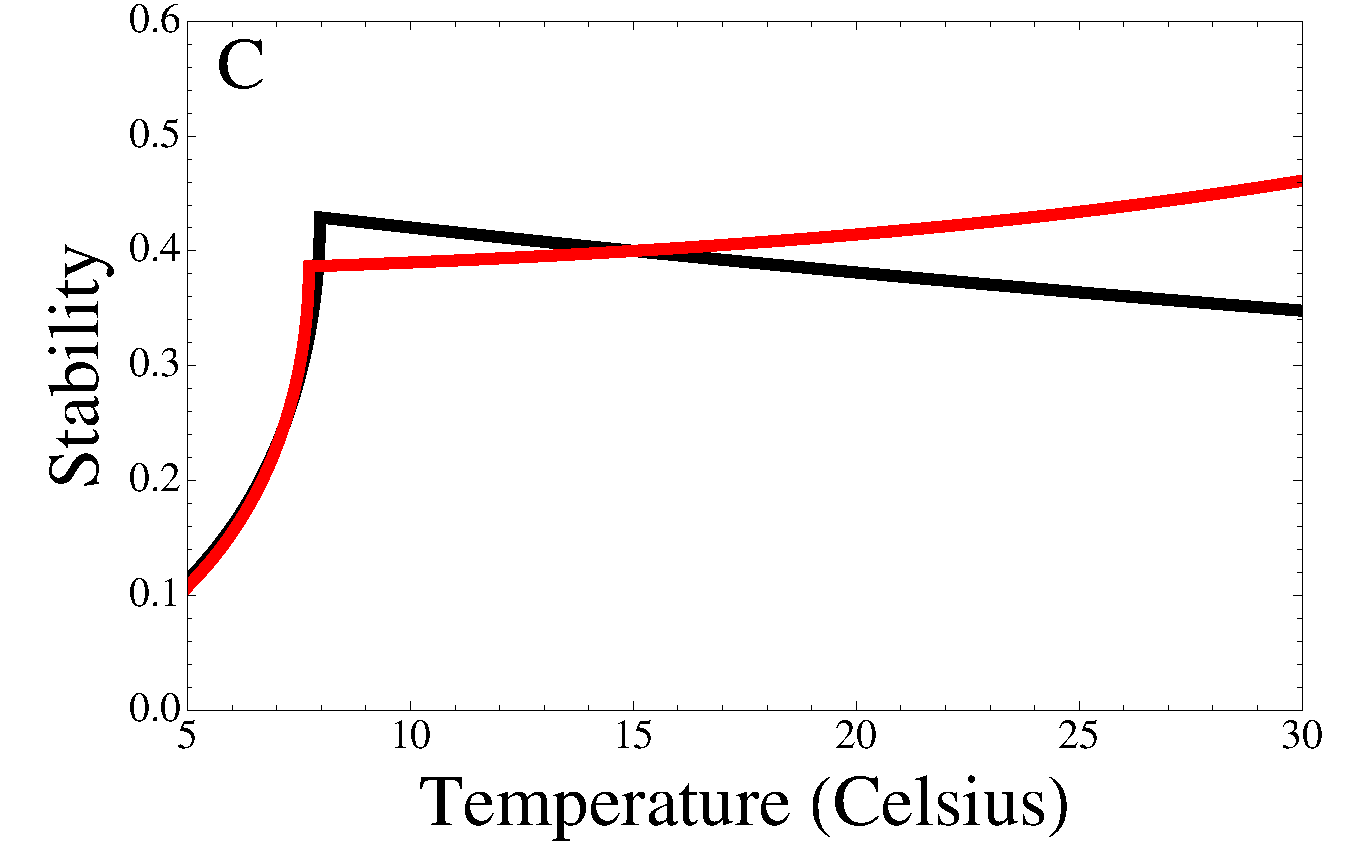
\includegraphics[width=0.5\linewidth]{StabilityAllTempMassDep}
\caption{
$B_{CR}$, equilibrium consumer to resource biomass ratio $\hat{C}:\hat{R}$, and stability of the coexistence equilibrium as functions of temperature $T$ (plotted in Celsius) with (red) and without (black) mass dependencies and the temperature-size rule.
Rate-constants (e.g., $r_0$) were chosen to make $r = 2$, $K = 100$, $a = 0.1$, $m = 0.6$, and $e = 0.15$ at 15$^\circ C$ (as in \cite{Gilbert2014}).
Other parameters as in \cite{Gilbert2014,DeLong2015}: $E_B = 0.32$ (solid dark), $E_B = 0.9$ (dashed and solid light), $E_S = 0.9$ (solid), $E_S = 0.32$ (dashed), $E_m = 0.65$, $E_{\nu,i} = 0.46$, $\nu_{0,i} = 1$, $\kappa = -0.81$, $\alpha = 1$, $\epsilon = -0.5$, $\mu = -0.29$, $\rho = -0.81$, $\beta_i = 0.02$ (red), $\beta_i = 0$ (black).  
}
\label{AllTempMassDep}
\end{figure}

%%%%%%%%%%%%%%%%%%%%%%%%%%%%%%%%%%%%%%%%%%%%%%%%
\begin{figure}[!ht]
\centering
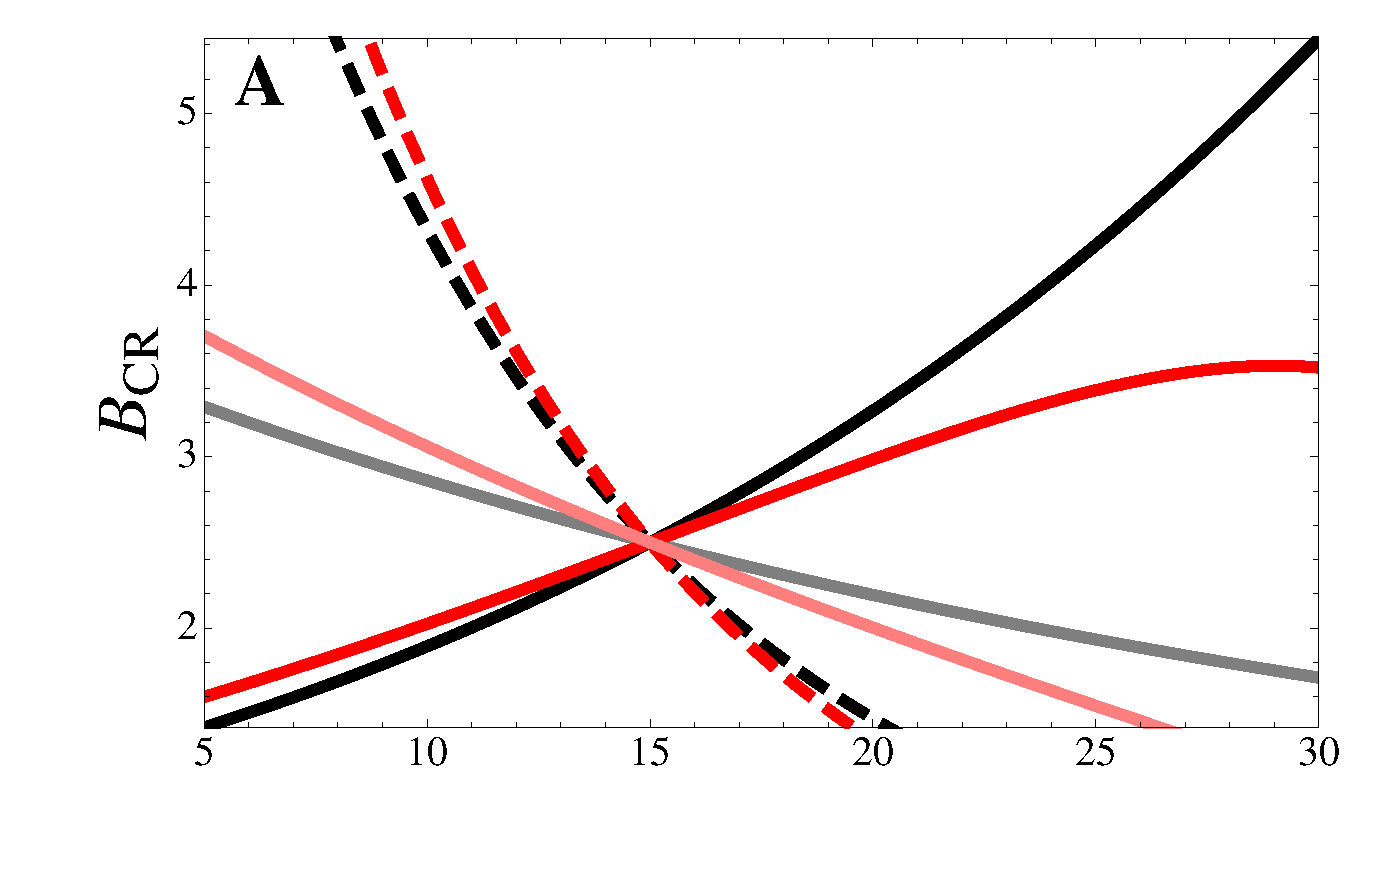
\includegraphics[width=0.5\linewidth]{BCRAllTempMassDepAsymm}
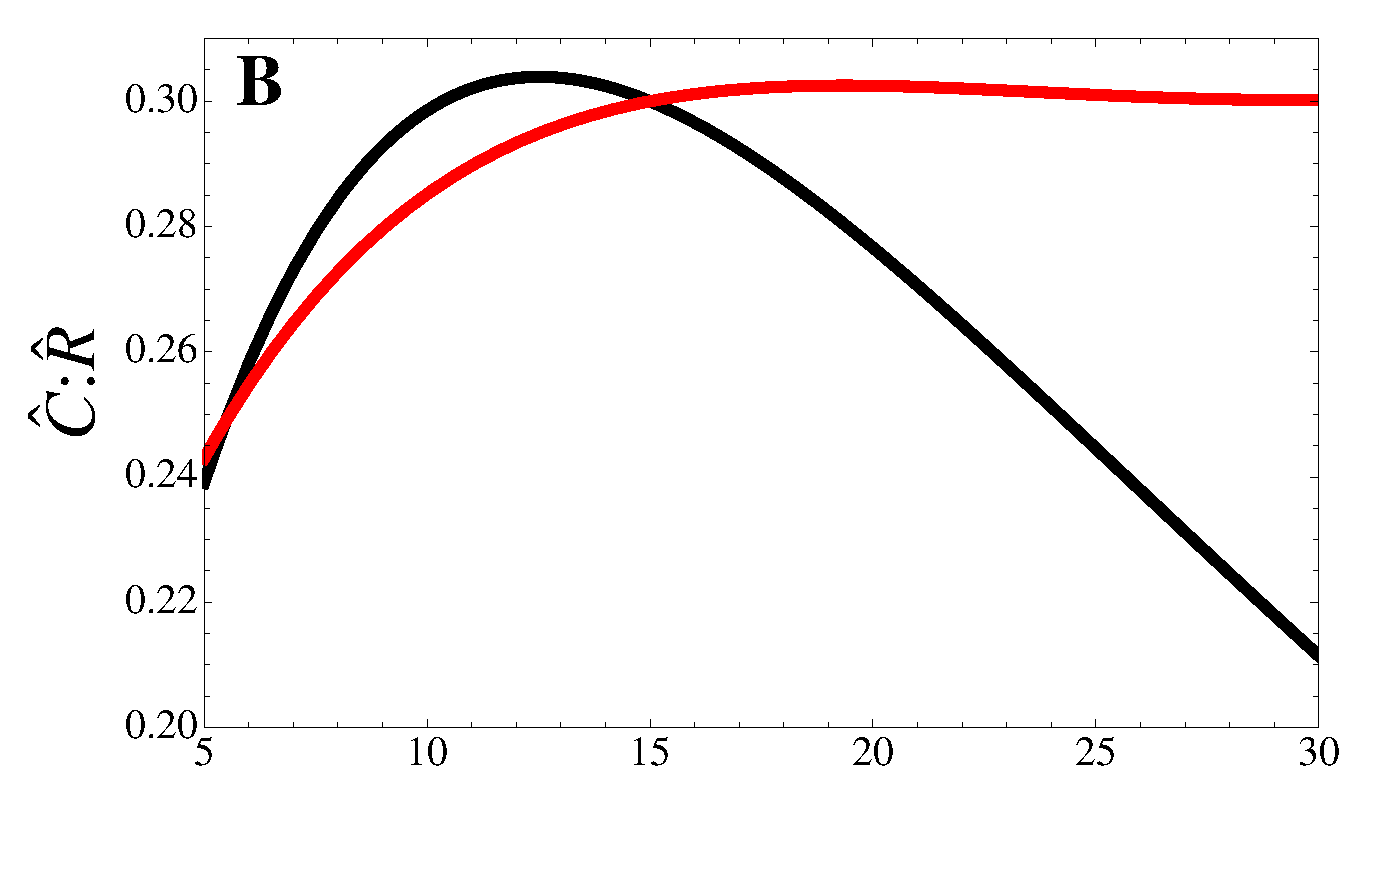
\includegraphics[width=0.5\linewidth]{CtoRAllTempMassDepAsymm}
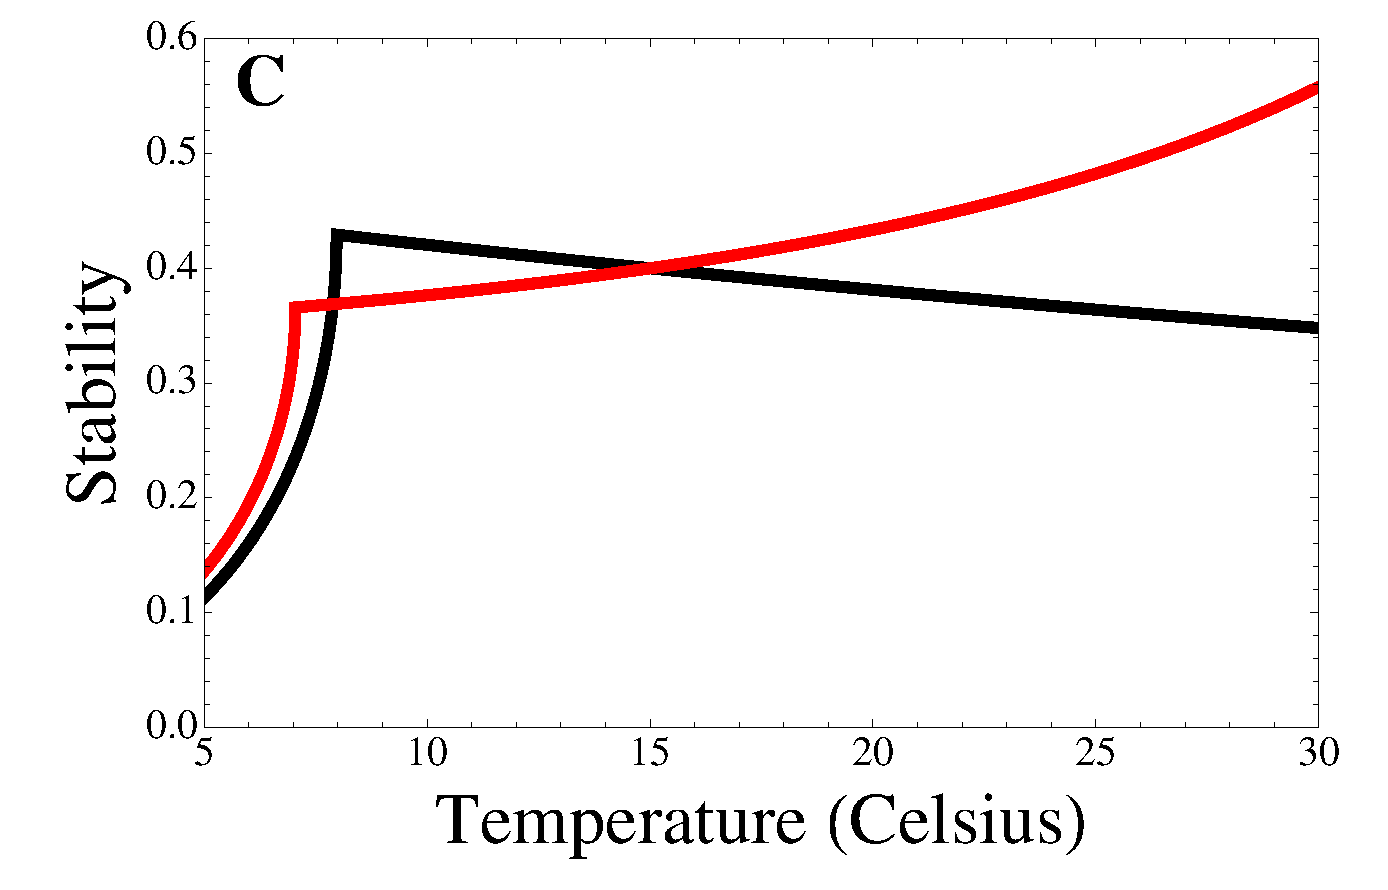
\includegraphics[width=0.5\linewidth]{StabilityAllTempMassDepAsymm}
\caption{
SUPPLEMENTARY FIGURE.
$B_{CR}$, equilibrium consumer to resource biomass ratio $\hat{C}:\hat{R}$, and stability of the coexistence equilibrium as functions of temperature $T$ (plotted in Celsius) with (red) and without (black) mass dependencies and the temperature-size rule.
Rate-constants (e.g., $r_0$) were chosen to make $r = 2$, $K = 100$, $a = 0.1$, $m = 0.6$, and $e = 0.15$ at 15$^\circ C$ (as in \cite{Gilbert2014}).
Other parameters as in \cite{Gilbert2014,DeLong2015}: $E_B = 0.32$ (solid dark), $E_B = 0.9$ (dashed and solid light), $E_S = 0.9$ (solid), $E_S = 0.32$ (dashed), $E_m = 0.65$, $E_{\nu,i} = 0.46$, $\nu_{0,i} = 1$, $\kappa = -0.81$, $\alpha = 1$, $\epsilon = -0.5$, $\mu = -0.29$, $\rho = -0.81$, $\beta_R = 0.02$ and $\beta_C = 0.04$ (red), $\beta_i = 0$ (black).  
}
\label{AllTempMassDepAsymm}
\end{figure}

%%%%%%%%%%%%%%%%%%%%%%%%%%%%%%%%%%%%%%%%%%%%%%%%
\begin{figure}[!ht]
\centering
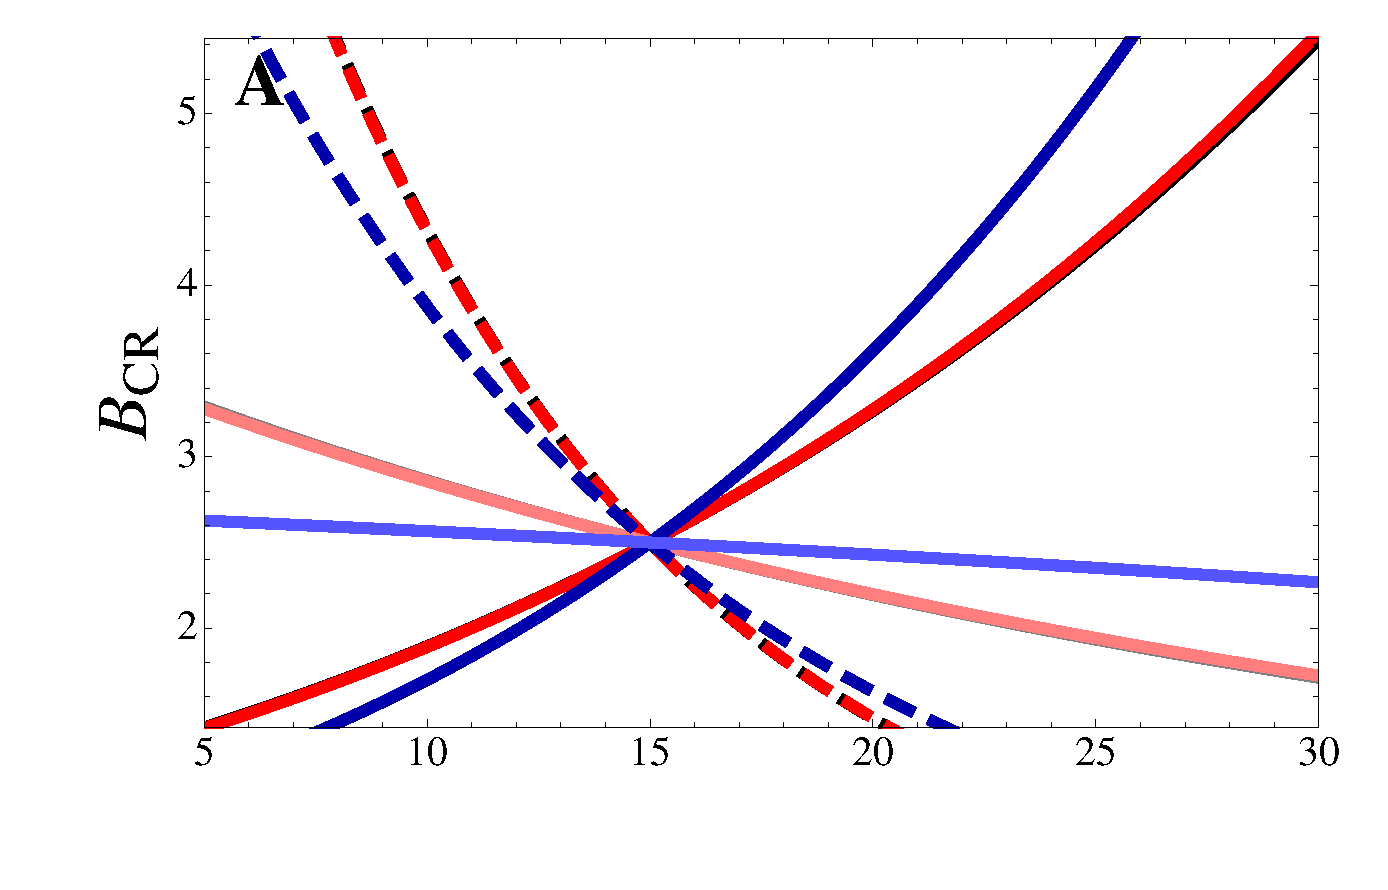
\includegraphics[width=0.5\linewidth]{BCRTypeII}
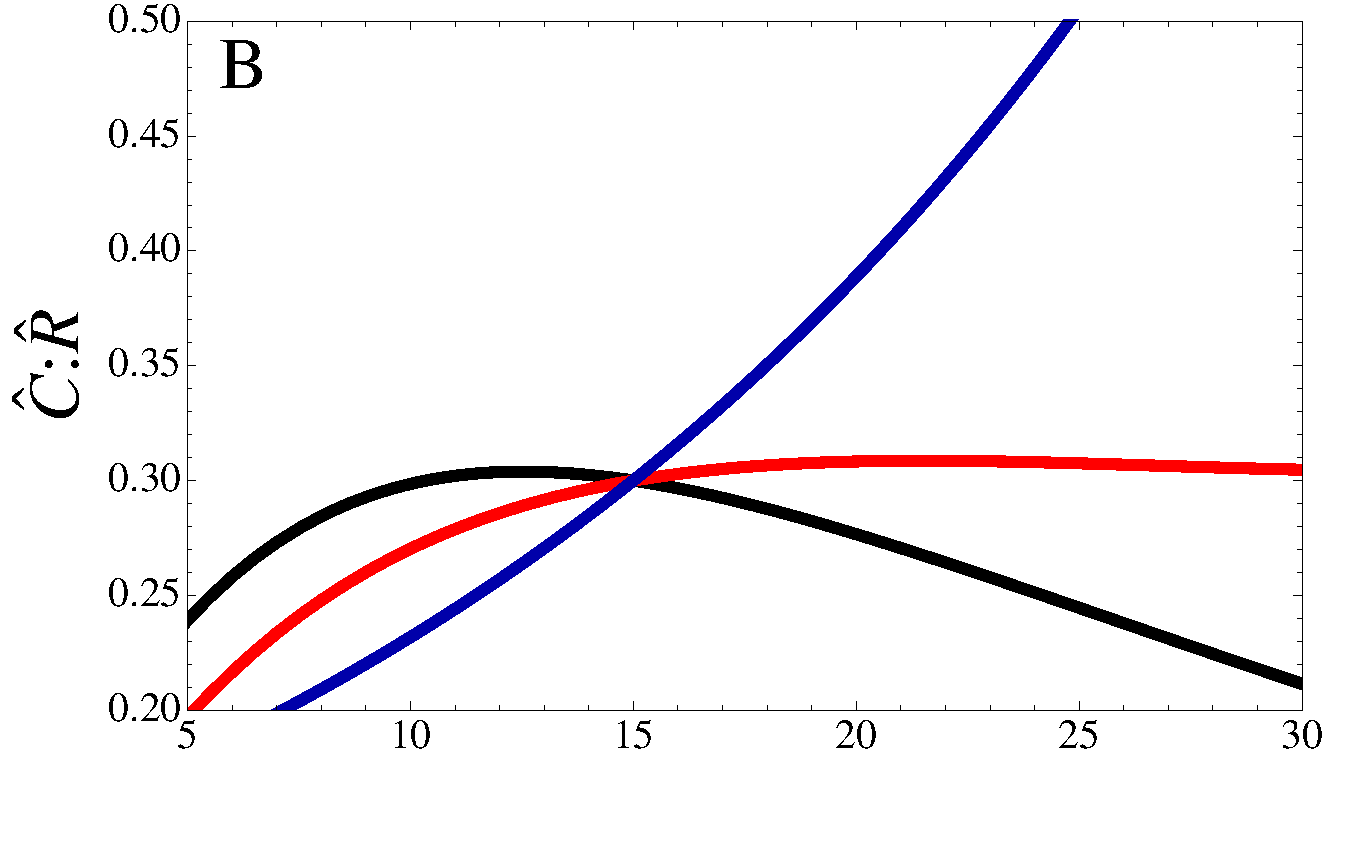
\includegraphics[width=0.5\linewidth]{CtoRTypeII}
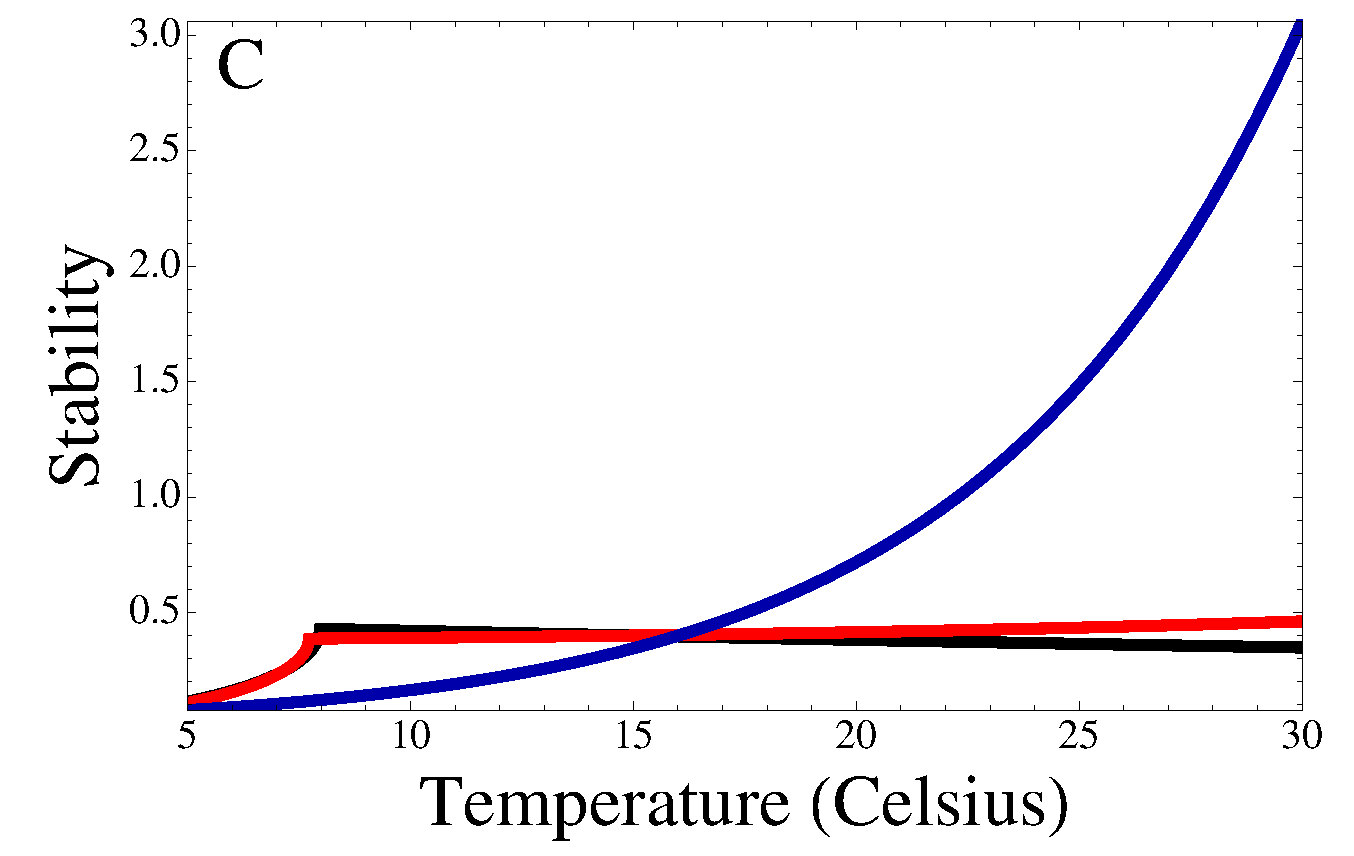
\includegraphics[width=0.5\linewidth]{StabilityTypeII}
\caption{
SUPPLEMENTARY FIGURE.
$B_{CR}$, equilibrium consumer to resource biomass ratio $\hat{C}:\hat{R}$, and stability of the coexistence equilibrium as functions of temperature $T$ (plotted in Celsius) with (red and blue) and without (black) mass dependencies and the temperature-size rule.
Type-II functional response in blue.
Rate-constants (e.g., $r_0$) were chosen to make $r = 2$, $K = 100$, $f(R) = 0.1$, $m = 0.6$, and $e = 0.15$ at 15$^\circ C$ (as in \cite{Gilbert2014}).
Other parameters as in \cite{Gilbert2014,DeLong2015,Rall2012}: $E_B = 0.32$ (solid dark), $E_B = 0.9$ (dashed and solid light), $E_S = 0.9$ (solid), $E_S = 0.32$ (dashed), $E_m = 0.65$, $E_{\nu,i} = 0.46$, $\nu_{0,i} = 1$, $\kappa = -0.81$, $\alpha = 1$, $\epsilon = -0.5$, $\mu = -0.29$, $\rho = -0.81$, $\beta_i = 0.02$ (red and blue), $\beta_i = 0$ (black), $a_C = 1/4+2/3$, $a_R = 1/3$, $h_C = -2/3$, $h_R = 0.5$, $E_a = 0.65$, $E_h = -0.65$, $h_0 = 10^{-13}$.  
}
\label{TypeII}
\end{figure}

%%%%%%%%%%%%%%%%%%%%%%%%%%%%%%%%%%%%%%%%%%%%%%%%
\begin{figure}[!ht]
\centering
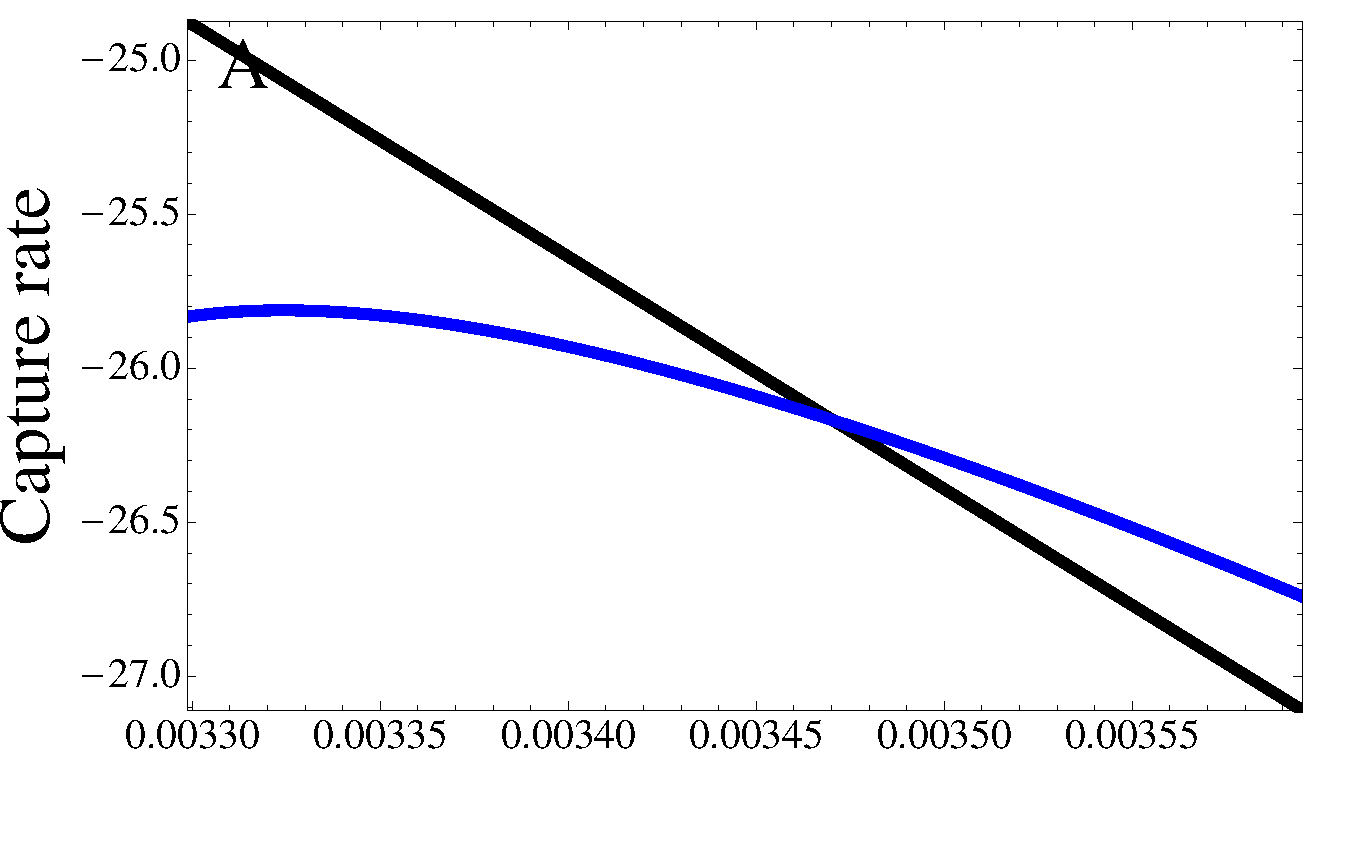
\includegraphics[width=0.5\linewidth]{CaptureTSRAsymm}
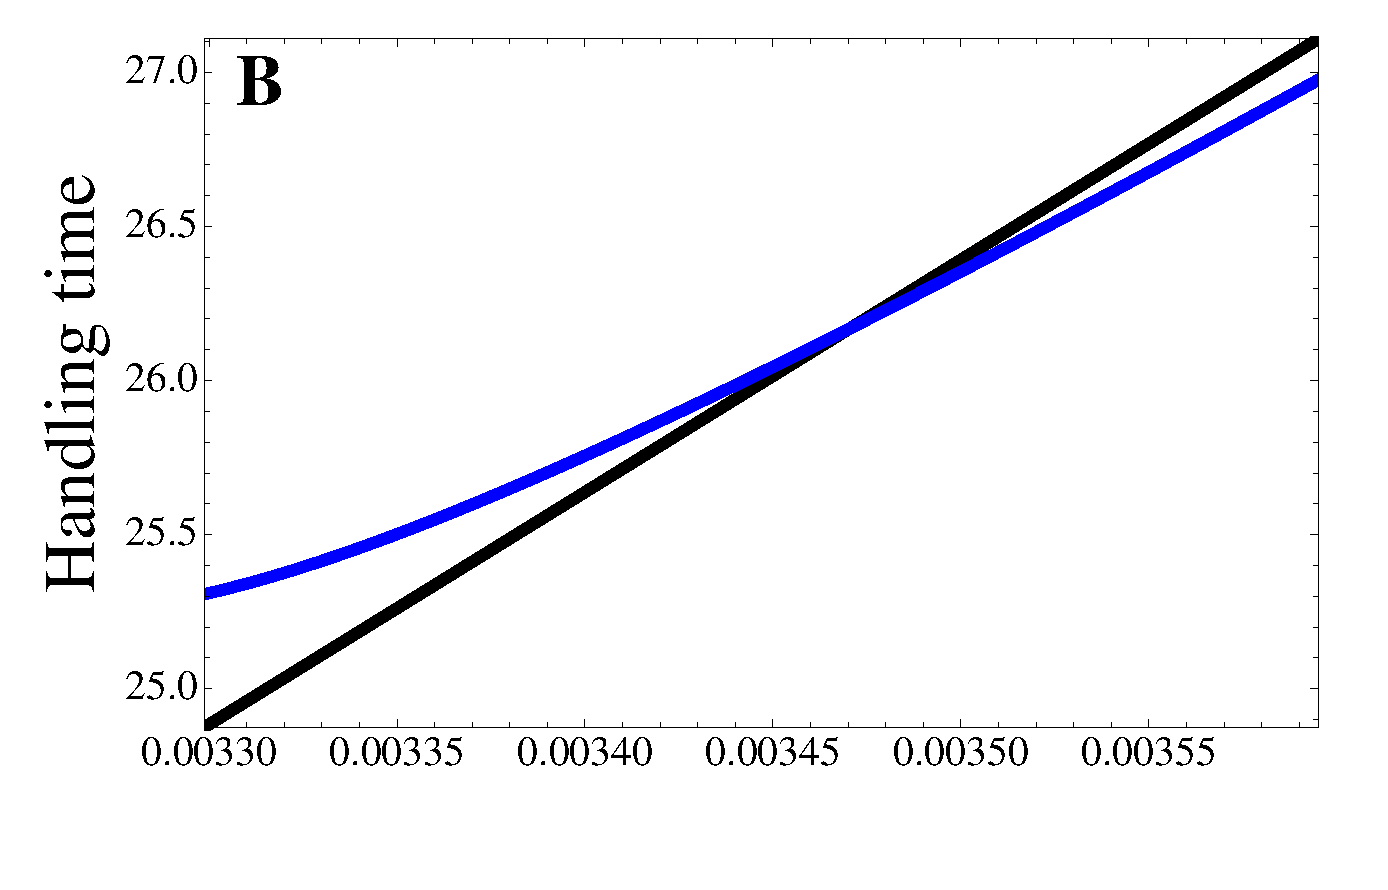
\includegraphics[width=0.5\linewidth]{HandlingTSRAsymm}
\caption{
SUPPLEMENTARY FIGURE.
The sensitivity of capture rate and handling time to temperature with (blue) and without (black) the temperature-size rule.
Plotted are (A) $\log(b/b0)$ and (B) $\log(h/h0)$.
Parameters as in \cite{Rall2012}: $a_C = 1/4+2/3$, $a_R = 1/3$, $h_C = -2/3$, $h_R = 0.5$, $E_a = 0.65$, $E_h = -0.65$.
}
\label{TypeII}
\end{figure}

\end{document}
